\documentclass[11pt, oneside]{article}   	% use "amsart" instead of "article" for AMSLaTeX format
\usepackage{geometry}                		% See geometry.pdf to learn the layout options. There are lots.
\geometry{a4paper}                   		% ... or a4paper or a5paper or ... 
%\geometry{landscape}                		% Activate for rotated page geometry
%\usepackage[parfill]{parskip}    		% Activate to begin paragraphs with an empty line rather than an indent
\usepackage{graphicx}				% Use pdf, png, jpg, or eps§ with pdflatex; use eps in DVI mode
								% TeX will automatically convert eps --> pdf in pdflatex		
\usepackage{amssymb}
\usepackage{amsmath}
%\usepackage{natbib}
\usepackage{filecontents}
\usepackage{graphicx}
\usepackage{caption} 
\usepackage{float}

%SetFonts

%SetFonts
\graphicspath{{figures/}}

\title{Benchmarking Algorithms for Short Text Classification}
\author{Raunak Agarwal, David Abraham, Nihal Gonsalves}
\date{}							% Activate to display a given date or no date

\begin{document}

%%%%%%%%%%%%%
%TITLE PAGE
%%%%%%%%%%%%%

\begin{titlepage}
\pagenumbering{gobble} 
\null  % Empty line
\nointerlineskip  % No skip for prev line
\vfill
\let\snewpage \newpage
\let\newpage \relax
\maketitle
\let \newpage \snewpage
\vfill 
\break % page break
\end{titlepage}


\pagenumbering{arabic}
\newpage
\tableofcontents
\newpage


%%%%%%%%%%%%%
%%%%%%%%%%%%%
%%%%%%%%%%%%%
%ABSTRACT
%%%%%%%%%%%%%
%%%%%%%%%%%%%
%%%%%%%%%%%%%


\section{Abstract}
The purpose of this paper is to present an empirical comparison of various classification techniques prevalent in the field of computational linguistics. It serves as a literature review of commonly used techniques in classifying short-text data. Short-text data, here, refers to any form of text-based data which has 10-20 words per data point, for example: chat data, tweets, Facebook comments, etc.
\\
The sentences are modelled using various word-representations: Continuous Bag-of-Words model, Skip-grams, Word2vec, etc. These representations work well on short-form text because of high accuracy on several similarity metrics. These representations are used as inputs to high-performance algorithms such as Support Vector Machines, Convolutional Neural Networks, Bi-directional LSTM's, etc. All the algorithms are subject to the same training and testing data under different domains. Further, the usage of pre-embedded vectors for word representations is explored.

%\subsection{}

%%%%%%%%%%%%%
%%%%%%%%%%%%%
%%%%%%%%%%%%%
%INTRODUCTION
%%%%%%%%%%%%%
%%%%%%%%%%%%%
%%%%%%%%%%%%%


\section{Introduction}
Natural Language Processing is the field of designing methods and algorithms to that input/output unstructured, natural language data. 
Text representation plays an important role in many NLP tasks such as document classification and clustering (Chen, 2017), document retrieval (Le & Mikolov, 2014), machine translation (Mikolov et al., 2013b), and multi-lingual document matching (Pham et al., 2015). Since there are no explicit features in text, much work has aimed to develop effective text representations. Among them, the simplest bag of words (BOW) approach (Salton & Buckley, 1988) and its term frequency variants (e.g. TF-IDF) (Robertson & Walker, 1994) are most widely used due to simplicity, efficiency and often surprisingly high accuracy (Wang & Manning, 2012). However, simply treating words and phrases as discrete symbols fails to take into account word order and semantics of the words

%%%%%%%%%%%%%
%%%%%%%%%%%%%
%%%%%%%%%%%%%
%LITERATURE REVIEW
%%%%%%%%%%%%%
%%%%%%%%%%%%%
%%%%%%%%%%%%%


\section{Literature Review}

%%%%%%%%%%%%%
%REPRESENTATIONS
%%%%%%%%%%%%%

\subsection{Representation}

The use of this data for research on text categorization requires a detailed understanding of the real world constraints under which the data was produced.It was essential that various preprocessing steps were taken in order to apply the training algorithm to the concerned text.This included 

Under the Hood :

\begin{enumerate}
	\item Logistic Regression  
	\item  Support Vector Classifiers
	\item Convolutional Neural Networks

\end{enumerate}

\subsubsection{CBOW}

Bag-of-words (BOW) representations contain information about the identities of all the ``words" (here, bigrams) of the document, without considering their order.
A Continuous Bag-of-Words representation can be created as: 
\begin{gather*}
\hat{y} = \frac{1}{\mid D \mid}\sum_{i=1}^{\mid D \mid} W^{D_{[i]}}
\end{gather*} where \begin{math} {\mid D \mid} \end{math}  is the total number of n-grams in the document \\

\subsubsection{skip-grams}

\subsubsection{Topic Modelling}
To perform classification using bag-of-words (BOW) model as features, gensim \cite{gensim} offers  a good framework. But the feature vectors of short text represented by BOW can be very sparse. And the relationships between words with similar meanings are ignored as well. One of the way to tackle this is to use topic modeling, i.e. representing the words in a topic vector. This package provides the following ways to model the topics:

LDA (Latent Dirichlet Allocation)
LSI (Latent Semantic Indexing)
RP (Random Projections)


The optimal dimensionality of word embeddings is mostly task-dependent: a smaller dimensionality works better for more syntactic tasks such as named entity recognition (Melamud et al., 2016) [44] or part-of-speech (POS) tagging (Plank et al., 2016) [32], while a larger dimensionality is more useful for more semantic tasks such as sentiment analysis (Ruder et al., 2016) [45].

\newpage
\subsubsection{Word2vec}

word2vec is the subject of two papers by Mikolov et al. in 2013. As word embeddings are a key building block of deep learning models for NLP, word2vec is often assumed to belong to the same group. Technically however, word2vec is not be considered to be part of deep learning, as its architecture is neither deep nor uses non-linearities.
In their first paper \cite{Mikolov1}, Mikolov et al. propose two architectures for learning word embeddings that are computationally less expensive than previous models. In their second paper \cite{Mikolov2}, they improve upon these models by employing additional strategies to enhance training speed and accuracy. These architectures the language model to take additional context into account.
\\
\textbf{Continuous bag-of-words (CBOW): }
While a language model is only able to look at the past words for its predictions, as it is evaluated on its ability to predict each next word in the corpus, a model that just aims to generate accurate word embeddings does not suffer from this restriction. Mikolov et al. thus use both the `n' words before and after the target word `w' to predict it as depicted in Figure \ref{fig:cbow}. 

They call this continuous bag-of-words (CBOW), as it uses continuous representations whose order is of no importance.

\begin{figure}[H]
\centering
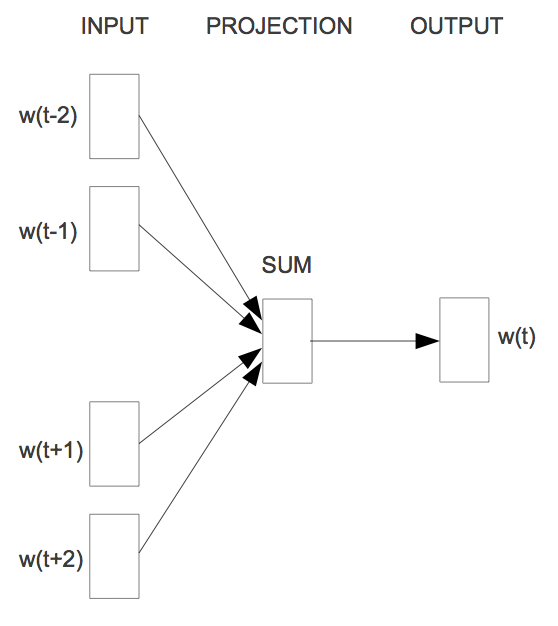
\includegraphics[width=0.4\linewidth]{cbow}
\caption{Continuous bag-of-words Architecture for word2vec}
\label{fig:cbow}
\end{figure}

Loss Function:
\begin{math}
J_\theta = \frac{1}{T}\sum\limits_{t=1}^T\ \text{log} \space p(w_t \: | \: w_{t-n} , \cdots , w_{t-1}, w_{t+1}, \cdots , w_{t+n})
\end{math}
\\Instead of feeding n previous words into the model, the model receives a window of n words around the target word w at each time step t.


\textbf{Skip-gram:}
While CBOW can be seen as a precognitive language model, skip-gram turns the language model objective on its head: Instead of using the surrounding words to predict the centre word as with CBOW, skip-gram uses the centre word to predict the surrounding words as can be seen in Figure \ref{fig:skip-gram}.

\begin{figure}[H]
\centering
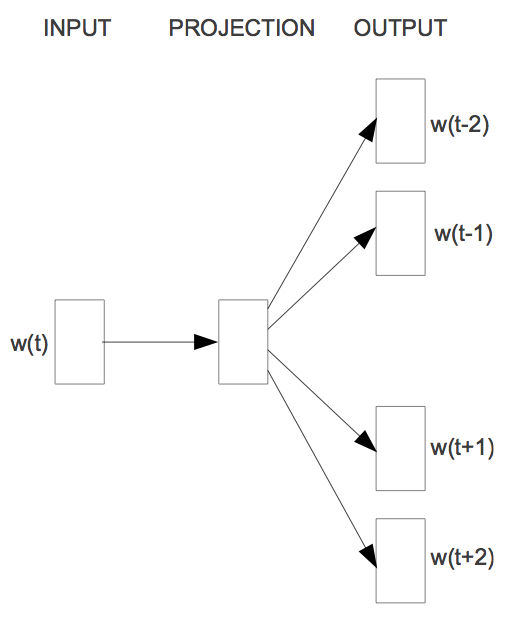
\includegraphics[width=0.4\linewidth]{skip-gram}
\caption{Skip-gram Architecture for word2vec}
\label{fig:skip-gram}
\end{figure}

The skip-gram objective thus sums the log probabilities of the surrounding n words to the left and to the right of the target word wt to produce the following loss function:
\begin{math}
\begin{centering}
J_\theta = \frac{1}{T}\sum\limits_{t=1}^T\ \sum\limits_{-n \leq j \leq n , \neq 0} \text{log} \space p(w_{t+j} \: | \: w_t)
\end{math}
\newline


\textbf{word2vec Summarised:}

Pros:
\begin{itemize}
	\item Dense semantic encoding
	\item A good representation framework
	\item Facilitates computation (similarity measure)
\end{itemize}

Cons:
\begin{itemize}
	\item Perform poorly for rare words and new words
\end{itemize}




%%%%%%%%%%%%%
%CLASSIFICATION
%%%%%%%%%%%%%
\newpage
\subsection{Classification}

CNN is mostly applied to image recognition thanks to the tolerance on translations (rotations, distortions) and the compositionality principle (entities are composed by its constituents). CNN might appear counter-intuitive at a first approach because text looks very different from images: The order of the words in text is not as important as the order of the pixel in an image, in addition, humans percept text sequentially, not in convolutions.

%todo


\begin{figure}[H]
\centering
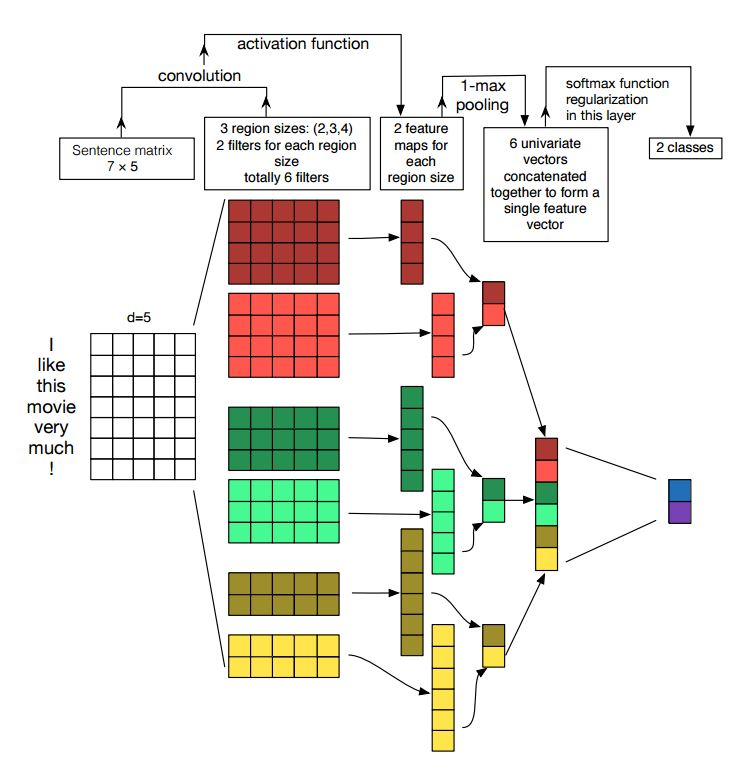
\includegraphics[width=0.8\linewidth]{TextCNN}
\caption{Convolutional Neural Network for Text}
\label{fig:TextCNN}
\end{figure}


\newpage
\section{Implementation}



%%%%%%%%%%%%%
%RESULTS
%%%%%%%%%%%%%

\newpage
\section{Results}


%%%%%%%%%% TRAVEL %%%%%%%%%%
\subsection{Travel Dataset}

%Support Vector Classifier with Pretrained Vectors%

\begin{table}[h]
\caption{Classification Report for SVC on the Travel Dataset}
\centering
\begin{tabular}{c | c c c c}
Class & Precision & Recall & F-score & Support\\
\hline
\hline\\
gotoPlace & 0.54 & 0.88 & 0.67 & 8\\
placeAccommodation & 1.0 & 1.0 & 1.0 & 7\\
placeExplore & 0.93 & 0.61 & 0.74 & 23\\
placeInformation & 0.73 & 0.85 & 0.79 & 13\\
placeLogistics & 0.88 & 1.0 & 0.93 & 7\\
avg & 0.84 & 0.79 & 0.79 & 58\\
\end{tabular}
\end{table}

\begin{figure}[h]
\centering
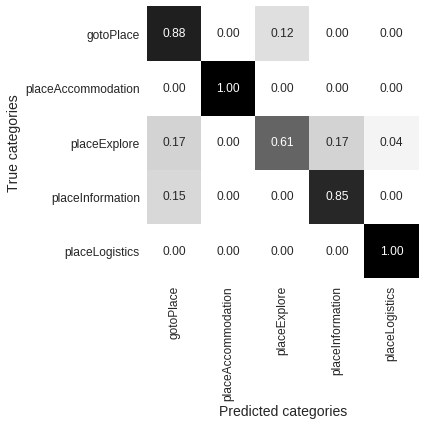
\includegraphics[width=0.6\linewidth]{SVC-Travel}
\caption{Confusion Matrix for SVC-Travel }
\label{fig:SVC-Travel}
\end{figure}

% CNN
\newpage
\begin{table}[h]
\caption{Classification Report for CNN on the Travel Dataset}
\centering
\begin{tabular}{c | c c c c}
Class & Precision & Recall & F-score & Support\\
\hline
\hline\\
gotoPlace & 0.67 & 0.75 & 0.71 & 8\\
placeAccommodation & 1.0 & 1.0 & 1.0 & 7\\
placeExplore & 0.95 & 0.83 & 0.88 & 23\\
placeInformation & 0.79 & 0.85 & 0.81 & 13\\
placeLogistics & 0.88 & 1.0 & 0.93 & 7\\
avg & 0.87 & 0.86 & 0.86 & 58\\
\end{tabular}
\end{table}

\begin{figure}[h]
\centering
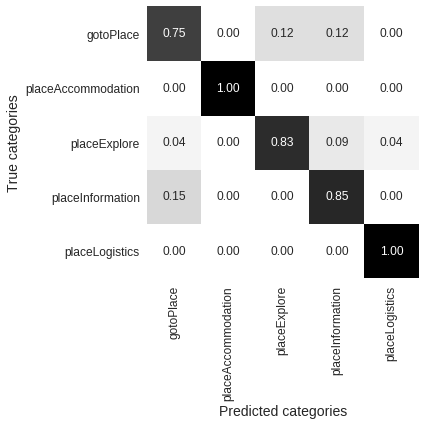
\includegraphics[width=0.6\linewidth]{CNN-Travel}
\caption{Confusion Matrix for CNN-Travel }
\label{fig:CNN-Travel}
\end{figure}

%Conv-LSTM
\newpage
\begin{table}[h]
\centering
\caption{Classification Report for Conv-LSTM on the Travel Dataset}
\begin{tabular}{c | c c c c}
Class & Precision & Recall & F-score & Support\\
\hline
\hline\\
gotoPlace & 1.0 & 0.75 & 0.86 & 8\\
placeAccommodation & 0.7 & 1.0 & 0.82 & 7\\
placeExplore & 0.88 & 0.91 & 0.89 & 23\\
placeInformation & 0.85 & 0.85 & 0.85 & 13\\
placeLogistics & 0.8 & 0.57 & 0.67 & 7\\
avg & 0.86 & 0.84 & 0.84 & 58\\
\end{tabular}
\end{table}

\begin{figure}[h]
\centering
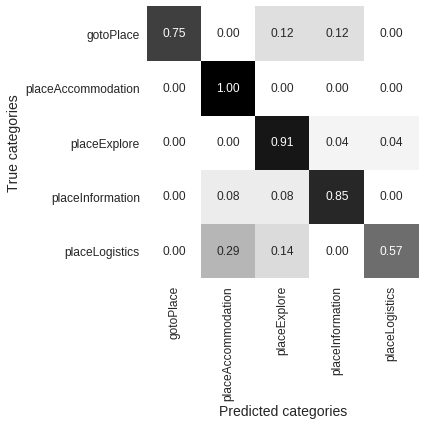
\includegraphics[width=0.6\linewidth]{ConvLSTM-Travel}
\caption{Confusion Matrix for ConvLSTM-Travel }
\label{fig:ConvLSTM-Travel}
\end{figure}

%Double-CNN
\newpage
\begin{table}[h]
\centering
\caption{Classification Report for Double-CNN on the Travel Dataset}
\begin{tabular}{c | c c c c}
Class & Precision & Recall & F-score & Support\\
\hline
\hline\\
gotoPlace & 0.18 & 1.0 & 0.3 & 8\\
placeAccommodation & 0.67 & 0.29 & 0.4 & 7\\
placeExplore & 1.0 & 0.26 & 0.41 & 23\\
placeInformation & 1.0 & 0.31 & 0.47 & 13\\
placeLogistics & 0.0 & 0.0 & 0.0 & 7\\
avg & 0.73 & 0.34 & 0.36 & 58\\
\end{tabular}
\end{table}

\begin{figure}[h]
\centering
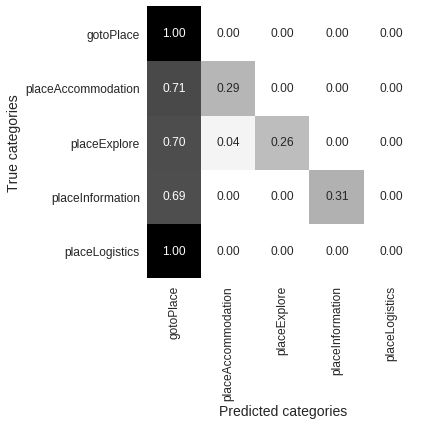
\includegraphics[width=0.6\linewidth]{DCNN-Travel}
\caption{Confusion Matrix for DCNN-Travel}
\label{fig:DCNN-Travel}
\end{figure}



%%%%%%%%%%%%%%%%ASK UBUNTU %%%%%%%%%%%%%%%%%%
\newpage
\subsection{Ask Ubuntu Dataset}

%SVC
\begin{table}[h]
\centering
\caption{Classification Report for CNN on the AskUbuntu Dataset}
\begin{tabular}{c | c c c c}
Class & Precision & Recall & F-score & Support\\
\hline
\hline\\
Make Update & 0.91 & 1.0 & 0.95 & 10\\
None & 0.0 & 0.0 & 0.0 & 1\\
Setup Printer & 1.0 & 1.0 & 1.0 & 5\\
Shutdown Computer & 0.88 & 0.88 & 0.88 & 8\\
Software Recommendation & 0.89 & 0.89 & 0.89 & 9\\
avg & 0.88 & 0.91 & 0.89 & 33\\
\end{tabular}
\end{table}

\begin{figure}[h]
\centering
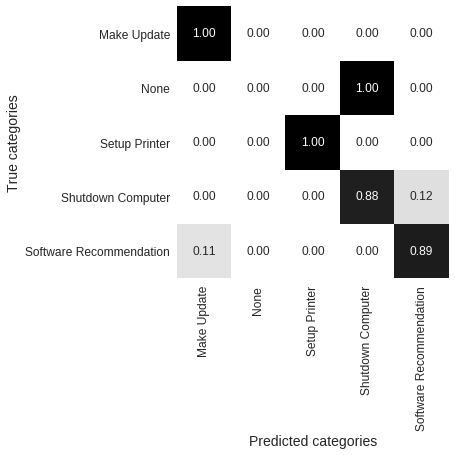
\includegraphics[width=0.6\linewidth]{SVC-AskUbuntu}
\caption{Confusion Matrix for SVC-AskUbuntu}
\label{fig:SVC-AskUbuntu}
\end{figure}

%CNN
\newpage
\begin{table}[h]
\centering
\caption{Classification Report for CNN on the AskUbuntu Dataset}
\begin{tabular}{c | c c c c}
Class & Precision & Recall & F-score & Support\\
\hline
\hline\\
Make Update & 1.0 & 1.0 & 1.0 & 13\\
None & 0.0 & 0.0 & 0.0 & 1\\
Setup Printer & 1.0 & 1.0 & 1.0 & 5\\
Shutdown Computer & 1.0 & 1.0 & 1.0 & 3\\
Software Recommendation & 0.92 & 1.0 & 0.96 & 11\\
avg & 0.94 & 0.97 & 0.96 & 33\\
\end{tabular}
\end{table}

\begin{figure}[h]
\centering
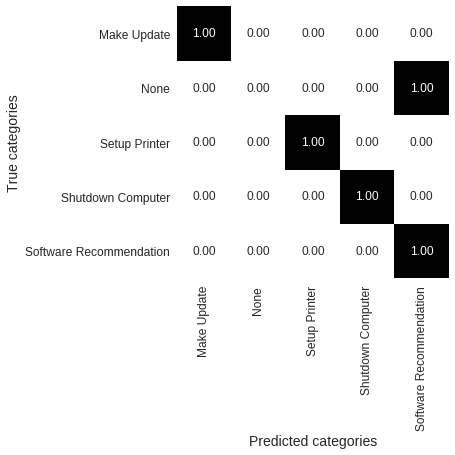
\includegraphics[width=0.6\linewidth]{CNN-AskUbuntu}
\caption{Confusion Matrix for CNN-AskUbuntu}
\label{fig:CNN-AskUbuntu}
\end{figure}


%CLSTM
\newpage
\begin{table}[h]
\centering
\caption{Classification Report for Conv-LSTM on the AskUbuntu Dataset}
\begin{tabular}{c | c c c c}
Class & Precision & Recall & F-score & Support\\
\hline
\hline\\
Make Update & 1.0 & 0.77 & 0.87 & 13\\
None & 0.0 & 0.0 & 0.0 & 1\\
Setup Printer & 1.0 & 1.0 & 1.0 & 5\\
Shutdown Computer & 1.0 & 1.0 & 1.0 & 3\\
Software Recommendation & 0.73 & 1.0 & 0.85 & 11\\
avg & 0.88 & 0.88 & 0.87 & 33\\
\end{tabular}
\end{table}

\begin{figure}[h]
\centering
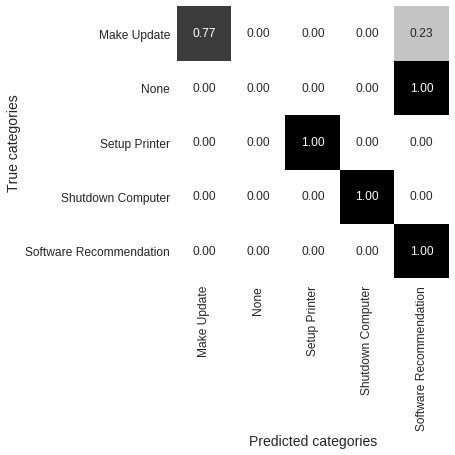
\includegraphics[width=0.6\linewidth]{ConvLSTM-AskUbuntu}
\caption{Confusion Matrix for ConvLSTM-AskUbuntu}
\label{fig:ConvLSTM-AskUbuntu}
\end{figure}


%DCNN
\newpage
\begin{table}[h]
\centering
\caption{Classification Report for Double-CNN on the AskUbuntu Dataset}
\begin{tabular}{c | c c c c}
Class & Precision & Recall & F-score & Support\\
\hline
\hline\\
Make Update & 1.0 & 0.69 & 0.82 & 13\\
None & 0.0 & 0.0 & 0.0 & 1\\
Setup Printer & 1.0 & 1.0 & 1.0 & 5\\
Shutdown Computer & 1.0 & 1.0 & 1.0 & 3\\
Software Recommendation & 0.69 & 1.0 & 0.81 & 11\\
avg & 0.87 & 0.85 & 0.84 & 33\\
\end{tabular}
\end{table}

\begin{figure}[h]
\centering
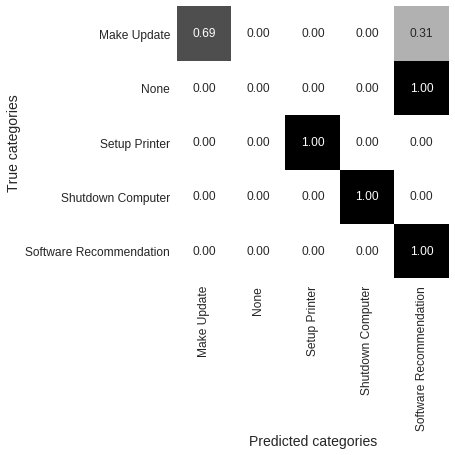
\includegraphics[width=0.6\linewidth]{DCNN-AskUbuntu}
\caption{Confusion Matrix for DCNN-AskUbuntu}
\label{fig:DCNN-AskUbuntu}
\end{figure}

%%%%%%%%%% HATE SPEECH %%%%%%%%%%%
\newpage
\subsection{Hate Speech Dataset}

%SVC
\begin{table}[h]
\centering
\caption{Classification Report for SVC on the Hate Speech Dataset}
\begin{tabular}{c | c c c c}
Class & Precision & Recall & F-score & Support\\
\hline
\hline\\
hate speech & 0.44 & 0.09 & 0.15 & 290\\
neither & 0.82 & 0.77 & 0.79 & 835\\
offensive & 0.9 & 0.96 & 0.93 & 3832\\
avg & 0.86 & 0.88 & 0.86 & 4957\\
\end{tabular}
\end{table}

\begin{figure}[h]
\centering
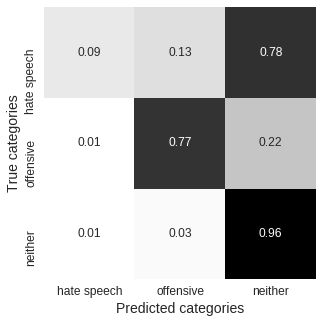
\includegraphics[width=0.6\linewidth]{SVC-HateSpeech}
\caption{Confusion Matrix for SVC-HateSpeech}
\label{fig:SVC-HateSpeech}
\end{figure}


%CNN
\newpage
\begin{table}[h]
\centering
\caption{Classification Report for CNN on the Hate Speech Dataset}
\begin{tabular}{c | c c c c}
Class & Precision & Recall & F-score & Support\\
\hline
\hline\\
hate speech & 0.31 & 0.2 & 0.25 & 286\\
neither & 0.7 & 0.69 & 0.69 & 838\\
offensive & 0.89 & 0.92 & 0.9 & 3833\\
avg & 0.82 & 0.84 & 0.83 & 4957\\
\end{tabular}
\end{table}

\begin{figure}[h]
\centering
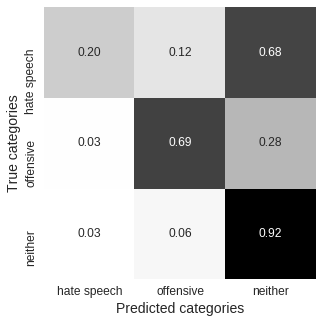
\includegraphics[width=0.6\linewidth]{CNN-HateSpeech}
\caption{Confusion Matrix for CNN-HateSpeech}
\label{fig:CNN-HateSpeech}
\end{figure}


%C-LSTM
\newpage
\begin{table}[h]
\centering
\caption{Classification Report for C-LSTM on the Hate Speech Dataset}
\begin{tabular}{c | c c c c}
Class & Precision & Recall & F-score & Support\\
\hline
\hline\\
hate speech & 0.27 & 0.12 & 0.17 & 286\\
neither & 0.72 & 0.72 & 0.72 & 838\\
offensive & 0.89 & 0.93 & 0.91 & 3833\\
avg & 0.82 & 0.84 & 0.83 & 4957\\
\end{tabular}
\end{table}

\begin{figure}[h]
\centering
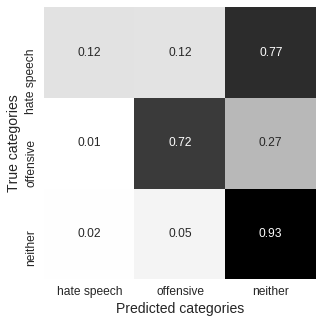
\includegraphics[width=0.6\linewidth]{ConvLSTM-HateSpeech}
\caption{Confusion Matrix for ConvLSTM-HateSpeech}
\label{fig:ConvLSTM-HateSpeech}
\end{figure}

% DCNN %
\newpage
\begin{table}[h]
\centering
\caption{Classification Report for DCNN on the Hate Speech Dataset}
\begin{tabular}{c | c c c c}
Class & Precision & Recall & F-score & Support\\
\hline
\hline\\
hate speech & 0.39 & 0.1 & 0.15 & 290\\
neither & 0.6 & 0.76 & 0.67 & 835\\
offensive & 0.9 & 0.89 & 0.89 & 3832\\
avg & 0.82 & 0.82 & 0.81 & 4957\\
\end{tabular}
\end{table}

\begin{figure}[h]
\centering
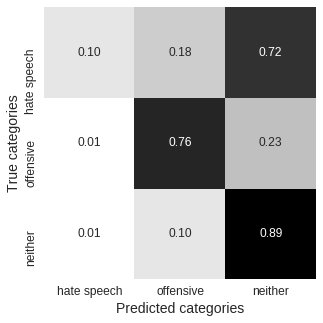
\includegraphics[width=0.6\linewidth]{DCNN-HateSpeech}
\caption{Confusion Matrix for DCNN-HateSpeech}
\label{fig:DCNN-HateSpeech}
\end{figure}

%%%%%%%%%%%%%%%  WEB APPLICATION CORPUS %%%%%%%%%%%%%%%
\newpage
\subsection{Web App Corpus}

%SVC
\begin{table}[h]
\centering
\caption{Classification Report for SVC on the Web App Corpus}
\begin{tabular}{c | c c c c}
Class & Precision & Recall & F-score & Support\\
\hline
\hline\\
Change Password & 1.0 & 1.0 & 1.0 & 2\\
Delete Account & 1.0 & 0.75 & 0.86 & 4\\
Export Data & 0.5 & 1.0 & 0.67 & 1\\
Filter Spam & 1.0 & 1.0 & 1.0 & 1\\
Find Alternative & 0.71 & 1.0 & 0.83 & 5\\
None & 0.0 & 0.0 & 0.0 & 1\\
Sync Accounts & 1.0 & 0.75 & 0.86 & 4\\
avg & 0.84 & 0.83 & 0.82 & 18\\
\end{tabular}
\end{table}

\begin{figure}[h]
\centering
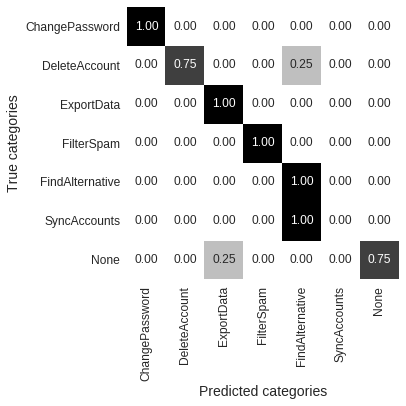
\includegraphics[width=0.5\linewidth]{SVC-WebAppCorpus}
\caption{Confusion Matrix for SVC-WebAppCorpus}
\label{fig:SVC-WebAppCorpus}
\end{figure}


%CNN
\newpage
\begin{table}[h]
\centering
\caption{Classification Report for CNN on the Web App Dataset}
\begin{tabular}{c | c c c c}
Class & Precision & Recall & F-score & Support\\
\hline
\hline\\
Change Password & 0.0 & 0.0 & 0.0 & 2\\
Delete Account & 0.75 & 0.75 & 0.75 & 4\\
Download Video & 0.0 & 0.0 & 0.0 & 0\\
Export Data & 0.0 & 0.0 & 0.0 & 1\\
Filter Spam & 1.0 & 0.6 & 0.75 & 5\\
Find Alternative & 1.0 & 1.0 & 1.0 & 3\\
None & 0.0 & 0.0 & 0.0 & 1\\
Sync Accounts & 1.0 & 1.0 & 1.0 & 2\\
avg & 0.72 & 0.61 & 0.65 & 18\\
\end{tabular}
\end{table}

\begin{figure}[h]
\centering
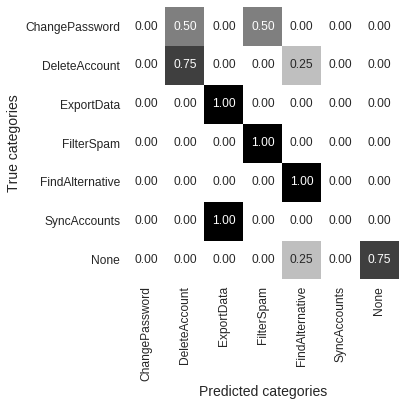
\includegraphics[width=0.5\linewidth]{CNN-WebAppCorpus}
\caption{Confusion Matrix for CNN-WebAppCorpus}
\label{fig:CNN-WebAppCorpus}
\end{figure}

%ConvLSTM
\newpage
\begin{table}[h]
\centering
\caption{Classification Report for ConvLSTM on the Web App Dataset}
\begin{tabular}{c | c c c c}
Class & Precision & Recall & F-score & Support\\
\hline
\hline\\
Change Password & 0.0 & 0.0 & 0.0 & 2\\
Delete Account & 1.0 & 0.75 & 0.86 & 4\\
Export Data & 1.0 & 1.0 & 1.0 & 1\\
Filter Spam & 1.0 & 1.0 & 1.0 & 1\\
Find Alternative & 1.0 & 0.8 & 0.89 & 5\\
None & 0.0 & 0.0 & 0.0 & 1\\
Sync Accounts & 0.75 & 0.75 & 0.75 & 4\\
avg & 0.78 & 0.67 & 0.72 & 18\\
\end{tabular}
\end{table}

\begin{figure}[h]
\centering
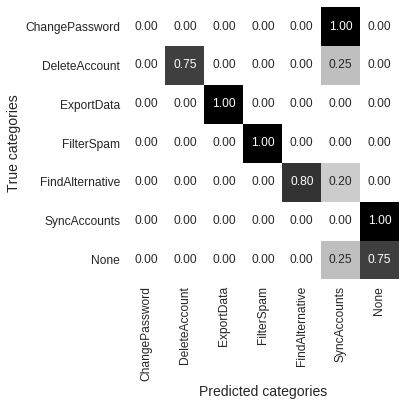
\includegraphics[width=0.6\linewidth]{ConvLSTM-WebAppCorpus}
\caption{Confusion Matrix for ConvLSTM-WebAppCorpus}
\label{fig:ConvLSTM-WebAppCorpus}
\end{figure}

%DCNN
\newpage
\begin{table}[h]
\centering
\caption{Classification Report for DoubleCNN on the Web App Dataset}
\begin{tabular}{c | c c c c}
Class & Precision & Recall & F-score & Support\\
\hline
\hline\\
Change Password & 0.0 & 0.0 & 0.0 & 2\\
Delete Account & 0.75 & 0.75 & 0.75 & 4\\
Export Data & 1.0 & 1.0 & 1.0 & 1\\
Filter Spam & 1.0 & 1.0 & 1.0 & 1\\
Find Alternative & 1.0 & 1.0 & 1.0 & 5\\
None & 0.0 & 0.0 & 0.0 & 1\\
Sync Accounts & 0.57 & 1.0 & 0.73 & 4\\
avg & 0.68 & 0.78 & 0.72 & 18\\
\end{tabular}
\end{table}

\begin{figure}[h]
\centering
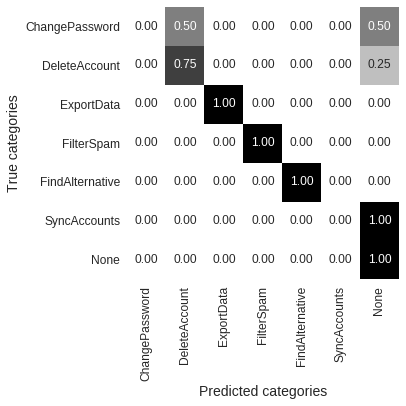
\includegraphics[width=0.6\linewidth]{DCNN-WebAppCorpus}
\caption{Confusion Matrix for DCNN-WebAppCorpus}
\label{fig:DCNN-WebAppCorpus}
\end{figure}

\newpage
\listoffigures

\newpage
\listoftables

\newpage
\nocite{*} 
\addcontentsline{toc}{section}{References}
\bibliography{review}
\bibliographystyle{plain}

\end{document}  